%!TEX root = ../Rnw_out/heartrate.tex
%$Header: /u/math/j40/cvsroot/data/0template/Rnw/template.Rnw.tex,v 1.1 2011/10/23 13:06:30 j40 Exp $

%$HeadURL: svn+ssh://gsawitzki@scm.r-forge.r-project.org/svnroot/rhrv/gs/Rnw/heartrate.Rnw $
%$Revision: 165 $
%$Date: 2014-08-23 22:39:14 +0200 (Sat, 23 Aug 2014) $
%svn propset svn:keywords "Date Author Id Revision HeadURL  Name" *.R

% -*- mode: noweb; noweb-default-code-mode: R-mode; -*-
%options(width=72);setwd( "/Users/gs/projects/rforge/rhrv/gs/Rnw_out");Sweave(file= "../Rnw/heartrate.Rnw", output="heartrate.tex", debug=TRUE, eps=FALSE, pdf=TRUE,  figs.only=FALSE)
%
%  Adjust the path names below and run the R command to process this file
%
%  cp <- tools::compactPDF("heartrate.pdf", gs_quality = "ebook")
%
%123
\typeout{Clear R workspace??}
%global flags for conditional builds
%:flags
\def\private{true}% comment out for public version
\def\solutions{true}% comment out to hide solutions
\def\usehyperref{true}% comment out to skip hyperref
\errorcontextlines=4%default:2

% S w eave material is commented out. So far, the file can be processed by plain LaTeX

\documentclass[a4paper, english, utf8]{amsart}
%\usepackage[applemac]{inputenc}
\usepackage[utf8]{inputenc}
\usepackage[english]{babel}
\usepackage{url} % used by natbib
\usepackage[square]{natbib} %[Azzalini & Bowman, 1990] 
% for \bibliographystyle{natdin}

%\usepackage{Sweave}%magic to avoid Sweave
\usepackage{gssda}
\usepackage{SIntro}
\usepackage[bookmarks, pdftex, 
pdftitle={Heart Rate Variability}, 
pdfauthor={G. Sawitzki},
colorlinks=true, linkcolor=black, citecolor=black, urlcolor=black, pdfpagemode=UseOC]{hyperref}
%pdfpagemode= UseNone UseOutlines UseThumbs FullScreen UseOC UseAttachments

\usepackage{graphics, colortbl}%for \rowcolor, \columncolor
\graphicspath{{./}{Rnw_out/}{media}{../media}}%Graetzer, p. 420

% \usepackage{gssda}
% \usepackage{colortbl}
% \usepackage{verbatim}        % small example code
% \usepackage{graphicx, fancyvrb, fancyref}
% %\graphicspath{{./}{./media/}{../media/}}%Graetzer, p. 420
\RequirePackage{graphicx,ae,fancyvrb}
\RequirePackage{longtable, varioref}

\newcommand{\figref}[1]{Figure\ \Vref{#1}}

\title{Estimating Heart Rate Variability}
\author[G. Sawitzki]{G\"unther Sawitzki}
\date{2014-02-20 (recovered)}
\email{\url{gs@statlab.uni-heidelberg.de}}
\address{\noindent G\"unther Sawitzki\newline
\indent StatLab Heidelberg\newline
\indent Im Neuenheimer Feld 294\newline
\indent D 69120 Heidelberg\newline}%\\\bigskip\bigskip\bigskip\bigskip\bigskip \\ %
%\keywords{data analysis, distribution diagnostics, recurrence plot}
\thanks{\emph{A waist book. These notes are an internal RFC for the R project RHRV, available from R-Forge. 
This is not for recirculation or general posting. 
These notes may contain copyrighted material from others. 
Copyrights have not been cleared. In particular material from RHRV may be used without explicit quotation. For all original references, see the source files in the Rforge repository.\\
\ \\
Corrections and comments are welcome.}\\
For more details on recurrence plots, see \cite{Sawitzki:2013recurrence}.\\
\indent \emph{Typeset}, with minor revisions: \today\  from svn $Revision: 165 $\\
\indent \url{gs@statlab.uni-heidelberg.de}
}%\\

%\affil...\endaffil
%\address...\endaddress
%\curraddr...\endcurraddr
%\urladdr...\endurladdr
%\thanks...\endthanks
%\dedicatory...\enddedicatory
%\translator...\endtranslator
%\keywords...\endkeywords
%\subjclass...\endsubjclass
%\abstract...\endabstract

%:Sweave
%\SweaveOpts{echo=TRUE}
%\newcommand\Stt[1]{\textsl{\texttt{#1}}}

%: layout
\RequirePackage{layouts} %used for LaTeX info only
%page layout for Sweave 6in plots
\addtolength{\textheight}{12mm}
\addtolength{\topmargin}{-9mm}   % still fits on US paper
%\addtolength{\textwidth}{26mm}   % still fits on US paper - 6.00612 in on A4
\setlength{\oddsidemargin}{20mm}
\setlength{\evensidemargin}{\oddsidemargin}

%  ****************************************
%  *           PARAGRAPHING               *
%  ****************************************
%
\parskip 12pt plus .25pt
\parindent 0pt %1em
\partopsep 2pt plus 1pt minus 1pt

%:Sweave
%\SweaveOpts{echo=TRUE}
\newcommand\Stt[1]{\textsl{\texttt{#1}}}
\renewcommand\urladdr[1]{\texttt{#1}}

%\usepackage{a4wide}

%%%%% from Sweave.sty
\setkeys{Gin}{width=0.8\textwidth}

\definecolor{sincol}{rgb}{0.0,0.0,0.8}% darkblue [r=0,   g=0,   b=.8]
\definecolor{soutcol}{rgb}{0.0,0.3,0.1}% darkgreen r=0.0,   g=.6, b=0]

\newcommand{\R}{{\normalfont\textsf{R}}{}}
\newcommand\code[1]{\textsl{\texttt{#1}}}
\newcommand\codex[1]{\textsl{\texttt{#1}}\index{#1@\texttt{#1}|textit}}


\makeindex
%\makenomenclature
\listfiles
%:{document}
\begin{document}
\maketitle
{\centering
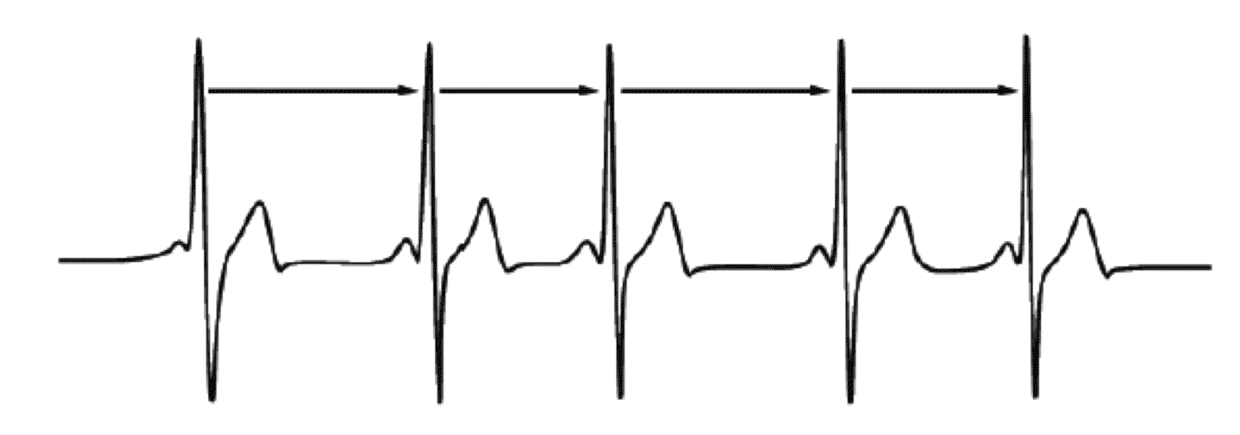
\includegraphics[width=0.6\linewidth]{../media/hrv1}

}
{
\parskip 0pt

\tableofcontents
}
\bigskip


\section{Purpose}
Heart rate variation is a non-invasive indicator of the physical state.
However, heart rate variation is a derived variable, based on heart
rate, and heart rate by itself is not an observable variable, but a
derived construct.

There are several sources that can be used to derive the heart rate. The
quality of the heart rate data, and hence the possibilities to 
assess the heart rate, depends on the quality of the original data and
the preprocessing steps.

The classical means is to register some form of pulse. In all of these,
classical methods the basic information is some local blood pressure, and the pulse
is derived from it. Typically this information is collected as an average
over a small number of beats ($\approx 15$ beats) or a small time interval (e.g. 15 s).

More precise information can be derived from ECG information. The ECG
records the potential difference between two or more electrodes at a
chosen sampling rate. Typical amplitudes range from -0.5mV to 2 mv. As
of 2014, the standard seems to be recording at 1024 Hz with 3 to 12 electrodes for 
clinical measurements. Technical
facilities allow ambulatory sampling for continuous time, typically using two electrodes.

In  clinical environment, the ECG recording is usually commented, and
the commenting annotations are an additional source of information
(\figref{fig:AnnECG}).
%12-Lead-ECG-showing-ST-Elevation-orange.jpg
\begin{figure}[htbp]
\begin{center}
\includegraphics[width=0.8\linewidth]{../media/12-Lead-ECG-showing-ST-Elevation-orange.jpg}

%\includegraphics[width=0.8\linewidth]{12-Lead-ECG-showing-ST-Elevation-orange.jpg}
\caption{Annotated ECG}
\label{fig:AnnECG}
\end{center}
\end{figure}


Heart rate, and heart rate variation are only means to judge the
physical state, and oxygen supply ported by the blood may be one of the
better indicators. Advanced devices can provide non-invasive measure of
the oxygen concentration. This combines information circulation and
respiration effects.

At present, we concentrate on ECG based data. These are common in
clinical environment, and in ambulatory devices as the Polar series of
monitors.

For evaluation, we concentrate on the RHRV package for R (version 4.0) \cite{RHRV-Mendez:2014aa}.

These technical notes concentrate on data preparation. Takens states and recurrence plots, with a view to heart rate variability, are discussed in a separate technical note \cite{Sawitzki:2013recurrence}.

\section{RHRV Data Import}

The data source for all ECG based data is an ECG recording. 
From this ECG recording, a beats data set is generated. 
Usually, pattern recognition is applied to detect QRS signals, and the 
time of the R component is reported as the beat time. 
This step may already include additional filtering.

RHRV can import various data formats. Section 5.2: ``Reading several
file formats'' of the RHRV tutorial gives some of the common
facilities. The LoadBeat function is a common interface for loading
heart beat data. In particular, \codex{LoadBeatAscii} loads an ASCII file with the time of beats, one beat per line. The time scale can be specified by the \code{scale} parameter of \code{LoadBeatAscii}.

The internal data is added to an extensible R list, a \codex{HRVData} structure in
terms of the RHRV tutorial (\cite{Garcia:2014aaTutorial}). At this point, the data
are a vector of  beat times [s], stored as a data frame (one variable) in component \code{\$Beat}.

\begin{Schunk}
\begin{Sinput}
> hrv.data  = CreateHRVData()
> hrv.data = SetVerbose(hrv.data, TRUE )
> hrv.data = LoadBeatAscii(hrv.data, "../beatsFolder/example.beats",
+        RecordPath = "../beatsFolder")
\end{Sinput}
\begin{Soutput}
** Loading beats positions for record: ../beatsFolder/example.beats **
   Path: ../beatsFolder 
   Scale: 1 
   Date: 01/01/1900
   Time: 00:00:00
   Number of beats: 17360 
\end{Soutput}
\end{Schunk}

The data structure is augmented by derived information in a second step (see Section 4.1.2 ``Calculating HR and filtering'' of \cite{Garcia:2014aaTutorial}).
\begin{Schunk}
\begin{Sinput}
> hrv.data = BuildNIHR(hrv.data)
\end{Sinput}
\begin{Soutput}
** Calculating non-interpolated heart rate **
   Number of beats: 17360 
\end{Soutput}
\end{Schunk}

At this point, the data are as given in Table \ref{tab:inventory} and contained it the \code{Beat} component of the \code{HRVData} list. The data structure maintained by \code{RHRV} may contain additional information.

\begin{table}
\begin{center}
\begin{tabular}{|l|p{0.5\linewidth}|l|}
\hline
\rowcolor[gray]{0.8}%
Name&Variable&Unit, Remarks\\
\hline
Time&beat time&[s]\\
niHR&(single beat) heart rate&[beats/min] (rounded?)\\
RR&beat duration&[ms]  (rounded?)\\
\hline
\end{tabular}
\end{center}
\caption{Raw data inventory}\label{tab:inventory}
\end{table}

There may be beats missing, due to the previous processing steps, and there may be gremlins that are 
generated by false events from the signal detection. An additional step may remove  some of the gremlins. 
\code{FilterNIHR} uses adaptive thresholds for rejecting those beats different from the given threshold 
more than a certain value. The rule for beat acceptation or rejection is to compare with previous, following 
and with the updated mean. It also applies a comparison with acceptable physiological values (default 
values 25 and 200 bpm). Details can be controlled by parameters for \code{FilterNIHR}. The data 
structure is similar to  \Vref{tab:inventory}, 
but the semantics has changed (\Vref{tab:inventoryfilt}).

\begin{table}
\begin{center}
\begin{tabular}{|l|p{0.5\linewidth}|l|}
\hline
\rowcolor[gray]{0.8}%
Name&Variable&Unit, Remarks\\
\hline
Time&beat time. Note: some beats have been filtered.&[s]\\
niHR&(single beat) heart rate&[beats/min] (??? rounded?)\\
RR&beat duration&[ms]  (??? rounded?)\\
\hline
\end{tabular}
\end{center}
\caption{Data inventory for filtered data}\label{tab:inventoryfilt}
\end{table}

\begin{Schunk}
\begin{Sinput}
> hrvfilt.data = FilterNIHR(hrv.data)
\end{Sinput}
\begin{Soutput}
** Filtering non-interpolated Heart Rate **
   Number of original beats: 17360 
   Number of accepted beats: 17259 
\end{Soutput}
\end{Schunk}

As a convenience, an interpolated version of the data can be provided to allow frequency domain analysis. But note: we are not dealing with stationary processes.

%# Note that it is not necessary to specify freqhr since it matches with
%# the default value: 4 Hz
\begin{Schunk}
\begin{Sinput}
> hrvipl.data = InterpolateNIHR (hrvfilt.data, freqhr = 4)
\end{Sinput}
\begin{Soutput}
** Interpolating instantaneous heart rate **
   Frequency: 4Hz
   Number of beats: 17259 
   Number of points: 29594 
\end{Soutput}
\end{Schunk}

The data may be imbedded in a \code{RHRVData} structure as outlined in \figref{fig:completeHRVData}.


\begin{figure}[htbp]
\begin{center}
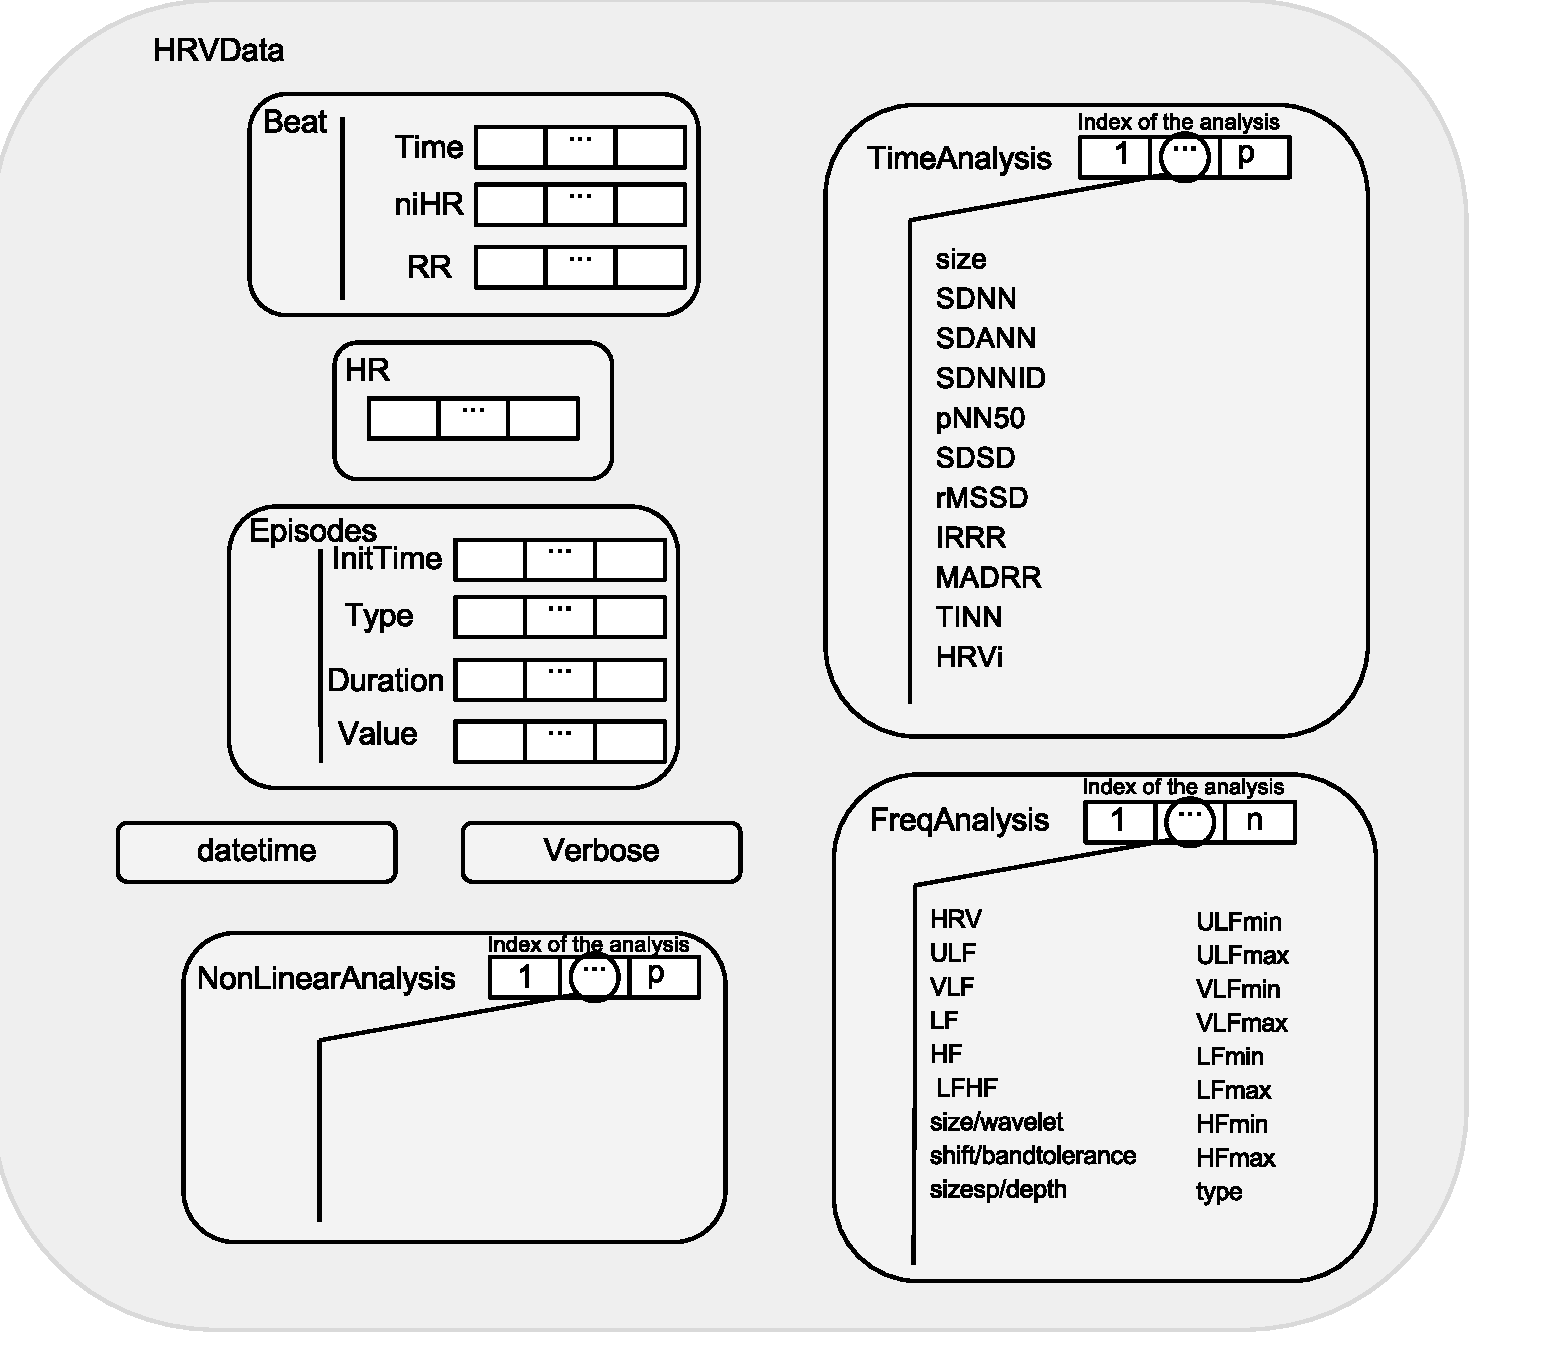
\includegraphics[width=0.8\linewidth]{../media/completeHRVData}
\caption{RHRV data structure: overview}
\label{fig:completeHRVData}
\end{center}
\end{figure}


\section{Support Functions}

These functions could go to RHRV.

\subsection{Plotsignal}
For signal representation, we use a common layout.
\todo{handle Beat not avail in plot}
\begin{Schunk}
\begin{Sinput}
> plotsignal <- function(signal, main, ylab) {
+ 	#! alpha level should depend on expected number of overlaps
+ 	
+ 	if (missing(ylab)) { ylab <- deparse(substitute(signal)) }
+ 
+ 	par(mfrow = c(1, 
+ 		2))
+ 	plot(signal, 
+ 		main = "", xlab = "index",  ylab = ylab,
+ 		col = rgb(0, 0, 1, 0.3), pch = 20)
+ 
+ 	plot(signal, type = "l", 
+ 		main = "",  xlab = "index", ylab = ylab,
+ 		col = rgb(0, 0, 0, 0.4))
+ 	points(signal, 
+ 		col = rgb(0, 0, 1, 0.3), pch = 20)
+ 	if (missing(main)) { main = deparse(substitute(signal)) }
+ 	title(main = main, 
+ 		outer = TRUE, line = -2, cex.main = 1.2)
+ }
\end{Sinput}
\end{Schunk}
\subsection{BuildNIDHR}


Since we are not interested in heart rate (or pulse), but in heart rate variation, a proposal is to use scaled differences
$$
HRRV_i = \frac{RR_i - RR_{i-1}}{(RR_i + RR_{i-1})/2}
$$
where $RR_i$ is the $i^{th}$ RR interval length. Taking these differences removes the mere pulse effects which otherwise may dominate the variation. There is no information loss, since the original RR sequence can be reconstructed, given initial conditions.

The residuals form this construct isolate structural influence from heart rate variation.

Note: if we think of online monitoring, statistics should be non-anticipating. We can take information from the past, as above, and should avoid assumptions about future data.


\begin{Schunk}
\begin{Sinput}
> # source('../../pkg/R/BuildNIHR2.R', chdir = TRUE)
> BuildNIDHR <-
+ function(HRVData, verbose=NULL) {
+ #------------------------------------------------------ 
+ # Obtains instantaneous heart rate variation from beats positions
+ # D for difference
+ #------------------------------------------------------ 
+ if (!is.null(verbose)) {
+ 	cat("  --- Warning: deprecated argument, using SetVerbose() instead ---\n",
+ 	    "--- See help for more information!! ---\n")
+ 	SetVerbose(HRVData,verbose)
+ }
+ 
+ if (HRVData$Verbose) {
+ 	cat("** Calculating non-interpolated heart rate differences **\n")
+ }
+ 
+ if (is.null(HRVData$Beat$Time)) {
+ 	cat("   --- ERROR: Beats positions not present... ",
+ 	"Impossible to calculate Heart Rate!! ---\n")
+ 	return(HRVData)
+ }
+ 
+ NBeats=length(HRVData$Beat$Time)
+ if (HRVData$Verbose) {
+ 	cat("   Number of beats:",NBeats,"\n");
+ }
+ 
+   # addition gs 
+    #using NA, not constant extrapolation as else in RHRV  
+    #drr=c(NA,NA,1000.0*	diff(HRVData$Beat$Time, lag=1 , differences=2))
+    HRVData$Beat$dRR=c(NA, NA, 
+    	1000.0*diff(HRVData$Beat$Time, lag=1, differences=2))
+ 
+    HRVData$Beat$avRR=(c(NA,HRVData$Beat$RR[-1])+HRVData$Beat$RR)/2
+    
+    HRVData$Beat$HRRV <- HRVData$Beat$dRR/HRVData$Beat$avRR
+ 
+ 	return(HRVData)
+ }
> 
> 
\end{Sinput}
\end{Schunk}
\clearpage

\section{First Inspection: example.beats}

\subsection{Hart Rate: example.beats}

\begin{Schunk}
\begin{Sinput}
> plotsignal(hrv.data$Beat$RR)
\end{Sinput}
\end{Schunk}
\begin{Schunk}
\begin{Sinput}
> plotsignal(hrvfilt.data$Beat$RR)
\end{Sinput}
\end{Schunk}

See \figref{fig:recurrence-hrvRR}
% for the unfiltered and \figref{fig:recurrence-hrvRRfilt} for the filtered version.

\todo{We have outliers at approximately 2*RR. 
Could this be an artefact of preprocessing, filtering out too many impulses?}
\begin{figure}[htbp]
\begin{center}
\includegraphics[width=0.8\linewidth]{heartrate-hrvRR}\\
\includegraphics[width=0.8\linewidth]{heartrate-hrvRRfilt}
\caption{RHRV tutorial example.beats. Signal and linear interpolation. Top: original version, bottom: fitered.}
\label{fig:recurrence-hrvRR}
\end{center}
\end{figure}

%\begin{figure}[htbp]
%\begin{center}
%\includegraphics[width=0.8\linewidth]{heartrate-hrvRRfilt}
%\caption{RHRV tutorial example.beats  filtered. Signal and linear interpolation.}
%\label{fig:recurrence-hrvRRfilt}
%\end{center}
%\end{figure}


\subsection{Hart Rate Variation: example beats}

If we are interested in heart rate variation, we may prefer starting with (scaled) differences.
\todo{Consider using differences}

\gsnote{differences for HRV}
\begin{Schunk}
\begin{Sinput}
> hrv.data <- BuildNIDHR(hrv.data)
\end{Sinput}
\begin{Soutput}
** Calculating non-interpolated heart rate differences **
   Number of beats: 17360 
\end{Soutput}
\begin{Sinput}
> HRRV <- hrv.data$Beat$HRRV
\end{Sinput}
\end{Schunk}
\index{heart rate variation}


\begin{Schunk}
\begin{Sinput}
> plotsignal(HRRV)
\end{Sinput}
\end{Schunk}
See \figref{fig:recurrence-hrvRRV},

\begin{figure}[htbp]
\begin{center}
\includegraphics[width=0.8\linewidth]{heartrate-hrvRRV}\\
\includegraphics[width=0.8\linewidth]{heartrate-hrvRRVfilt}
\caption{RHRV tutorial example.beats. HRRV Signal (differences) and linear interpolation.
Top: original version, bottom: fitered.
}
\label{fig:recurrence-hrvRRV}
\end{center}
\end{figure}

%
\begin{Schunk}
\begin{Sinput}
> hrvfilt.data <- BuildNIDHR(hrvfilt.data)
\end{Sinput}
\begin{Soutput}
** Calculating non-interpolated heart rate differences **
   Number of beats: 17259 
\end{Soutput}
\begin{Sinput}
> HRRVfilt <- hrvfilt.data$Beat$HRRV
\end{Sinput}
\end{Schunk}
\index{heart rate variation}


\begin{Schunk}
\begin{Sinput}
> plotsignal(HRRVfilt)
\end{Sinput}
\end{Schunk}
See \figref{fig:recurrence-hrvRRV},
%
%\begin{figure}[htbp]
%\begin{center}
%\includegraphics[width=0.8\linewidth]{heartrate-hrvRRVfilt}
%\caption{RHRV tutorial example.beats, filtered.  HRRV Signal (differences) and linear interpolation.}
%\label{fig:recurrence-hrvRRVfilt}
%\end{center}
%\end{figure}

\clearpage

\section{First Inspection: example2.beats}
\begin{Schunk}
\begin{Sinput}
> hrv2.data  = CreateHRVData()
> hrv2.data = SetVerbose(hrv2.data, TRUE )
> hrv2.data = LoadBeatAscii(hrv2.data, "example2.beats",
+        RecordPath = "../beatsFolder")
\end{Sinput}
\begin{Soutput}
** Loading beats positions for record: example2.beats **
   Path: ../beatsFolder 
   Scale: 1 
   Removed 2437 duplicated beats
   Date: 01/01/1900
   Time: 00:00:00
   Number of beats: 2437 
\end{Soutput}
\begin{Sinput}
> hrv2.data = BuildNIHR(hrv2.data)
\end{Sinput}
\begin{Soutput}
** Calculating non-interpolated heart rate **
   Number of beats: 2437 
\end{Soutput}
\begin{Sinput}
> hrv2filt.data = FilterNIHR(hrv2.data)
\end{Sinput}
\begin{Soutput}
** Filtering non-interpolated Heart Rate **
   Number of original beats: 2437 
   Number of accepted beats: 2434 
\end{Soutput}
\end{Schunk}

\subsection{Hart Rate example 2}
\begin{Schunk}
\begin{Sinput}
> plotsignal(hrv2.data$Beat$RR)
\end{Sinput}
\end{Schunk}
\begin{Schunk}
\begin{Sinput}
> plotsignal(hrv2filt.data$Beat$RR)
\end{Sinput}
\end{Schunk}
See \figref{fig:recurrence-hrvRR2}.
%  for the unfiltered and \figref{fig:recurrence-hrvRR2filt} for the filtered version.


\begin{figure}[htbp]
\begin{center}
\includegraphics[width=0.8\linewidth]{heartrate-hrvRR2}\\
\includegraphics[width=0.8\linewidth]{heartrate-hrvRR2filt}
\caption{RHRV tutorial example2.beats. Signal and linear interpolation.
Top: original version, bottom: fitered.} 
\label{fig:recurrence-hrvRR2}
\end{center}
\end{figure}

%\begin{figure}[htbp]
%\begin{center}
%\includegraphics[width=0.8\linewidth]{heartrate-hrvRR2filt}
%\caption{RHRV tutorial example2.beats filtered. Signal and linear interpolation.}
%\label{fig:recurrence-hrvRR2filt}
%\end{center}
%\end{figure}

\clearpage
\subsection{Hart Rate Variation: example2.beats}

\index{heart rate variation}

\begin{Schunk}
\begin{Sinput}
> hrv2.data <- BuildNIDHR(hrv2.data)
\end{Sinput}
\begin{Soutput}
** Calculating non-interpolated heart rate differences **
   Number of beats: 2437 
\end{Soutput}
\begin{Sinput}
> HRRV2 <- hrv2.data$Beat$HRRV
> plotsignal(HRRV2)
\end{Sinput}
\end{Schunk}
See \figref{fig:recurrence-hrvRRV2},

\begin{figure}[htbp]
\begin{center}
\includegraphics[width=0.8\linewidth]{heartrate-hrvRRV2}\\
\includegraphics[width=0.8\linewidth]{heartrate-hrvRRV2filt}
\caption{RHRV tutorial example2.beats. HRRV Signal (differences) and linear interpolation.
Top: original version, bottom: fitered.}
\label{fig:recurrence-hrvRRV2}
\end{center}
\end{figure}

%
\begin{Schunk}
\begin{Sinput}
> hrv2filt.data <- BuildNIDHR(hrv2filt.data)
\end{Sinput}
\begin{Soutput}
** Calculating non-interpolated heart rate differences **
   Number of beats: 2434 
\end{Soutput}
\begin{Sinput}
> HRRV2filt <- hrv2filt.data$Beat$HRRV
> plotsignal(HRRV2filt)
\end{Sinput}
\end{Schunk}
See \figref{fig:recurrence-hrvRRV2},
\index{heart rate variation}

%\begin{figure}[htbp]
%\begin{center}
%\includegraphics[width=0.8\linewidth]{heartrate-hrvRRV2filt}
%\caption{RHRV tutorial example2.beats, filtered. HRRV2 Signal (differences) and linear interpolation.}
%\label{fig:recurrence-hrvRRV2filt}
%\end{center}
%\end{figure}

\section{Exercises}
\begin{exca}
Augment the data structure to reflect filtering.
\end{exca}

\begin{exca}
For analysis of heart rate variability, we are interested in effect in the range of less than 10s.

Can you modify the displays to focus on this range?
\end{exca}

\begin{exca}
For analysis of recovery effects, we are interested in effect in the range of less about 5 min (??).

Can you modify the displays to focus on this range?
\end{exca}

%@
%:backmatter
\clearpage
\nocite{*}
\bibliographystyle{jss} % local
%\bibliographystyle{biblatex} % not natbib compatible
%\bibliographystyle{authordate3}% bib/din1505/alphadin.bst
%\bibliography{sda,../pulse}
\bibliography{../pulse}
%
\clearpage

\printindex

%\clearpage
%\renewcommand{\nomname}{Notation}
%%cleardoublepage%see nomencl, p. 7
%
%\printnomenclature %Nomenclature, used for notation table

\clearpage
\R{} session info:

Total Sweave time used: 11.078 sec. at Tue Aug 26 19:33:43 2014.

{\tiny
\begin{itemize}\raggedright
  \item R version 3.1.1 (2014-07-10), \verb|x86_64-apple-darwin13.1.0|
  \item Locale: \verb|en_GB.UTF-8/en_GB.UTF-8/en_GB.UTF-8/C/en_GB.UTF-8/en_GB.UTF-8|
  \item Base packages: base, datasets, graphics, grDevices,
    methods, stats, tcltk, utils
  \item Other packages: leaps~2.9, locfit~1.5-9.1, MASS~7.3-34,
    Matrix~1.1-5, mgcv~1.8-2, nlme~3.1-117,
    nonlinearTseries~0.2.2, rgl~0.94.1118, RHRV~4.0,
    sintro~0.1-3, tkrplot~0.0-23, TSA~1.01, tseries~0.10-32,
    waveslim~1.7.3
  \item Loaded via a namespace (and not attached): grid~3.1.1,
    lattice~0.20-29, quadprog~1.5-5, tools~3.1.1, zoo~1.7-12
\end{itemize}}

%\RequirePackage{layouts}
\LaTeX{} information:
{\tiny

\currentpage 
textwidth: \printinunitsof{in}\prntlen{\textwidth} \qquad 
linewidth:\printinunitsof{in}\prntlen{\linewidth}\\
textheight: \printinunitsof{in}\prntlen{\textheight}\\
}

Bibliography style: jss

CVS/Svn repository information:

{\tiny%
\noindent
\verb+$Source: /u/math/j40/cvsroot/lectures/src/dataanalysis/Rnw/recurrence.Rnw,v $+\\
\verb!$HeadURL: svn+ssh://gsawitzki@scm.r-forge.r-project.org/svnroot/rhrv/gs/Rnw/heartrate.Rnw $!\\
\verb+$Revision: 165 $+\\
\verb!$Date: 2014-08-23 22:39:14 +0200 (Sat, 23 Aug 2014) $!\\
\verb+$name:  $+\\
\verb+$Author: gsawitzki $+
}
\typeout{**** $Id: heartrate.Rnw 165 2014-08-23 20:39:14Z gsawitzki $ done ****}
\typeout{**** $HeadURL: svn+ssh://gsawitzki@scm.r-forge.r-project.org/svnroot/rhrv/gs/Rnw/heartrate.Rnw $ done ****}
\end{document}




%	%:Sweave examples
%	%<<print=TRUE>>=
%	%<<results=hide>>=
%	%@
%	%<<echo=TRUE,print=TRUE>>=
%	%<<>>=
%	%@
%	%%\texttt{x} is 6.28318530717959, the
%	%<<engine=R>>=
%	%@ %def
%	%\begin{figure}[htbp]
%	%  \begin{center}
%	%<<fig=TRUE>>=
%	%@
%	%    \caption{.}
%	%  \end{center}
%	%\end{figure}
%	%<<engine=S4>>=
%	%@
